\documentclass[../besoin_user.tex]{subfiles}
\begin{document}

\section{Menu principal}
\begin{figure}[h]
    \centering
    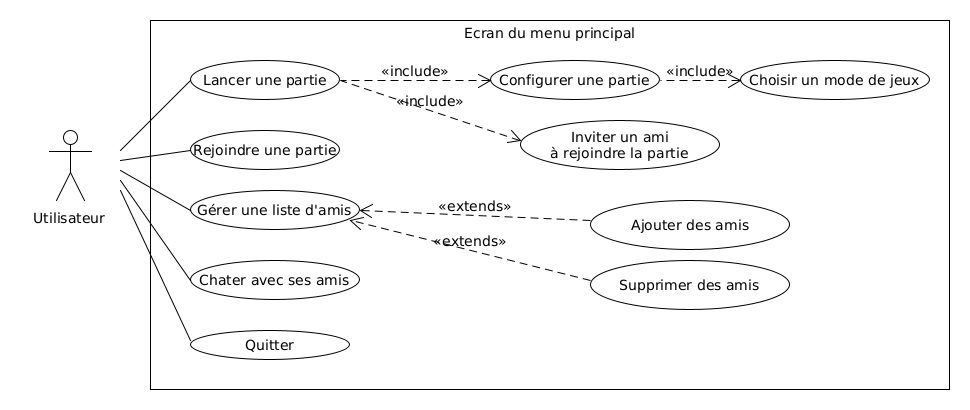
\includegraphics[scale=0.5]{img_fonctionnel/use_case_user_ecran_principal.png}
    \label{fig:user_menu_principal}
    \caption{Menu principal}
\end{figure}

\subsection{Lancement d'une partie}
Lors du lancement d'une partie le joueur doit simplement fixer les règles en choisissant :
\begin{itemize}
	\item[-] Le type de partie : \textbf{classique} ou \textbf{commandant}
	\item[-] Le temps d'une partie : au maximum \textbf{15 minutes}
	\item[-] Le temps par tour d'un joueur : au maximum \textbf{30 secondes}
\end{itemize}

Après quoi il sera redirigé vers un lobby, auquel il pourra inviter des joueurs, qui seront tous en mode spectateur s'ils acceptent l'invitation.
Un joueur peut aussi rejoindre le lobby sans recevoir d'invitation.
Si au moins un joueur à rejoint la partie, le joueur principale peut le fixer en tant que second joueur et lancer la partie.
Mais avant que la partie ne puisse commencer, il faudra placer tous les bateaux disponibles sur le board, après quoi la partie se lance.

\subsection{Rejoindre une partie}
Lorsqu'un utilisateur est invité par un ami a rejoindre une partie, il a la possibilité de rejoindre la partie en acceptant l'invitation, mais il peut aussi refuser
ou encore ignorer l'invitation. Si jamais le joueur est déconnecté, un message d'erreur est affiché pour informer qu'il n'est pas possible d'inviter le joueur.
Un joueur a aussi la possibilité de rejoindre une partie sans invitation à condition que la partie soit au stade de lobby.


\subsection{Gérer sa liste d'ami}
Chaque utilisateur possède une liste d'amis qu'il peut modifier. Il a la possibilité de:
\begin{itemize}
    \item ajouter un ami a sa liste
    \item retirer un ami de sa liste
\end{itemize}

\subsection{Chat}
Si le joueur a des amis en ligne dans sa liste d'amis, il a la possibilité de communiquer avec eux via un chat. 
Si un ami n'est pas connecté, ses messages cesseront d'être transmis, et le programme lui présentera un message l'informant de cette situation.
\end{document}